% eQoSystem, 2026 Global Quantum + AI Challenge, Phase 1 concept proposal
% Problem statement: E.ON, Quantum-Enabled Grid Expansion Planning for
% Distribution System Energy Networks.
% Formatting: A4, 10pt everywhere (the guidelines set 10pt as the minimum),
% at most 6 pages. Compile: pdflatex proposal.tex (twice).
\documentclass[10pt,a4paper]{article}
\usepackage[T1]{fontenc}
\usepackage[utf8]{inputenc}
\usepackage[margin=1.8cm,top=1.7cm,bottom=1.7cm]{geometry}
\usepackage{amsmath}
\let\Bbbk\relax
\usepackage{newtxtext,newtxmath}
\usepackage{graphicx}
\usepackage{booktabs}
\usepackage{tabularx}
\usepackage{multirow}
\usepackage{xcolor}
\usepackage{microtype}
\usepackage{enumitem}
\usepackage{titlesec}
\usepackage{caption}
\usepackage[hidelinks]{hyperref}
\usepackage{url}

\graphicspath{{figures/}}
\definecolor{eon}{RGB}{21,54,102}
\definecolor{q}{RGB}{33,102,172}

% headings: compact, coloured, numbered with the mandated section names
\titleformat{\section}{\color{eon}\bfseries\large}{\thesection.}{0.5em}{}
\titlespacing*{\section}{0pt}{9pt plus 2pt minus 2pt}{4pt}
\titleformat{\subsection}{\bfseries}{\thesubsection}{0.5em}{}
\titlespacing*{\subsection}{0pt}{6pt plus 1pt minus 1pt}{2pt}
\setlength{\parskip}{2.2pt}
\setlength{\parindent}{0pt}
\setlist[itemize]{nosep,leftmargin=1.2em,topsep=1pt}
\setlist[enumerate]{nosep,leftmargin=1.5em,topsep=1pt}
\captionsetup{font=normalsize,labelfont=bf,skip=3pt}
\renewcommand{\arraystretch}{1.08}
\pagestyle{plain}

% one place to edit the public repository link
\newcommand{\repourl}{https://github.com/AshrafBoussahi/eQoSystem-EON-GridExpansion}
\newcommand{\qgridxurl}{https://github.com/ashrafboussahi/qGridX}
\newcommand{\pypiurl}{https://pypi.org/project/qgridx/}
\newcommand{\blogurl}{https://www.aiqcommunity.org/news/q-volution-first-place}
\newcommand{\qvolrepo}{https://github.com/AshrafBoussahi/Rigetti_Quantum_Grid_Optimization_eQoSystem}
\newcommand{\hibarole}{team member; role and affiliation as entered in the portal team profile}

\begin{document}

% ---------------------------------------------------------------- header
\begin{center}
{\color{eon}\bfseries\Large Pauli Correlation Encoding for Distribution Grid
Expansion Planning}\\[3pt]
{\large Thousands of build-or-no-build line decisions on tens of qubits,
three measurement settings at any size, and a hardness ladder to benchmark
them on}\\[6pt]
{\bfseries Team eQoSystem} \quad (AiQC, Ai and Quantum Community)\\[2pt]
Achraf Boussahi (lead), Abir Chekroun, Zakaria Lourghi,
Mouadh Abderrahmane Assal, Hiba Menacer\\[2pt]
Lead contact: \href{mailto:ashraf@aiqcommunity.org}{ashraf@aiqcommunity.org}
\quad Public repository: \url{\repourl}\\[2pt]
Problem statement: \textbf{E.ON}, \emph{Quantum-Enabled Grid Expansion Planning
for Distribution System Energy Networks}
\end{center}
\vspace{2pt}
\hrule
\vspace{4pt}

\textbf{Summary.} E.ON's problem is combinatorial along one axis: the number of
build-or-no-build line decisions. That is exactly the axis along which the
standard one-qubit-per-variable quantum mapping fails, and exactly the axis
along which Pauli correlation encoding (PCE) is cheapest. PCE stores each
binary decision in the sign of a $k$-body Pauli correlation, so an $n$-qubit
register carries up to $3\binom{n}{k}$ decisions and, because the strings
split into three commuting families, the device runs three measurement
settings whatever the problem size. We have already built and published the
full workflow on transmission-planning problems with real power-flow
coefficients (45 decisions on 6 qubits, 105 on 7, 9,009 on 15), measured its
three-setting property on a 108-qubit superconducting processor, shown that
discrete native-gate PCE circuits beat variational PCE at low quantum budget
up to 858 variables on 13 qubits, and won first place globally in the Rigetti
advanced track of the Q-Volution hackathon with a PCE solution to a 180-node
grid optimisation problem. This proposal re-targets that stack at E.ON's
line-addition formulation, adds a QOBLIB-style hardness ladder of distribution
expansion instances, and commits to a Qiskit-executable, reproducible PoC with
numeric success criteria.

% ---------------------------------------------------------------- 1
\section{Problem Framing}

\textbf{Our reading of the problem.} A distribution system operator holds a
network $G=(V,E_0)$, a set of candidate additions $E_c$ (new ties, parallel
conductors, conductor upgrades on existing corridors), and a scenario set
$S$ of future operating conditions with probabilities $p_s$. The decision is
$x\in\{0,1\}^{m}$, $m=|E_c|$: which candidates to build. The objective E.ON
names is congestion, the amount by which line flows exceed ratings, summed
over lines and scenarios, traded against investment cost under a budget (a
two-objective structure of the kind treated in [6]). We
adopt the binary linear programming family of reference [4] of the challenge
statement, in which candidate lines are scored by their influence on
congested branches, and we keep the flow physics linear as in the demand
coincidence models of reference [1]:
\begin{equation}
\min_{x\in\{0,1\}^m}\;\sum_{s\in S}p_s\sum_{l\in E_0\cup E_c(x)}
\max\!\bigl(0,\,|f^{s}_{l}(x)|-F_l\bigr)\;+\;\lambda\sum_{e\in E_c}\kappa_e x_e
\quad\text{s.t.}\;\sum_{e}\kappa_e x_e\le K,\;\; x\in\mathcal{T},
\label{eq:problem}
\end{equation}
where $f^{s}_{l}(x)$ is the linearised flow on line $l$ in scenario $s$ given
the built set, $F_l$ the thermal rating, $\kappa_e$ the cost of candidate $e$,
$K$ the budget, and $\mathcal{T}$ the topology rules a DSO imposes (radial
operation of low-voltage feeders, at most one upgrade tier per corridor).
Outputs are the ones the statement asks for: the set of lines to build, the
objective value, and the congestion before and after. The formulation is
deliberately a variant of the network expansion literature rather than a new
invention; the challenge asks for hard instances of such a variant, and that is
where our contribution starts.

\textbf{Why the decision count is the barrier.} A medium-voltage subgrid with a
few hundred corridors and three upgrade options per corridor is already
$m\approx 10^3$. The mainstream quantum optimisation proposals (QAOA, VQE on an Ising
Hamiltonian, annealing) spend one qubit per binary variable, so
$m=10^3$ needs a thousand-qubit register at a fidelity no device offers today. The
gap is a property of the encoding, not of the hardware roadmap.

\textbf{Why PCE gives a credible route.} Pauli correlation encoding [7] reads
decision $i$ from the sign of the expectation value of a $k$-body Pauli string
$\Pi_i$ on an $n$-qubit state, $x_i=\tfrac12(1+\operatorname{sign}\langle\Pi_i\rangle)$.
Taking strings from the three uniform families $X^{\otimes k}$, $Y^{\otimes k}$
and $Z^{\otimes k}$ over qubit subsets gives capacity $m_{\max}=3\binom{n}{k}$:
45 decisions on 6 qubits, 105 on 7, 2,000 candidate lines on 18 qubits at
$k=3$ (capacity 2,448), and 4,500 on 14 qubits at $k=5$. Strings within a family commute, so
one basis rotation reads a whole family at once and the number of measurement
settings is three, independent of $m$ and $n$. Both properties have been
measured by us, not argued: Table~\ref{tab:evidence} lists what already runs.

\textbf{What a successful outcome would change for E.ON.} Today candidate
reinforcements are screened by rules and experience and iterated through
simulation, which is why plans tend to be conservative. A solver whose device
workload stays at three circuits while the candidate set grows into the
thousands lets a planner evaluate the joint choice over the whole candidate
set, across all scenarios, and return a ranked set of lines with the
congestion relief each delivers. We claim no quantum speed-up at the scale
where a mixed-integer solver certifies optima in milliseconds; we claim a
resource profile that is bounded along the axis on which the problem explodes,
and we propose to test it on instances certified to be hard.

\begin{table}[t]
\centering
\caption{What already runs, end to end, before the PoC starts. All numbers are
from our published result files (repository in the header). Rows 1 to 4 are
storage-siting and graph problems with the same quadratic form as
Eq.~\eqref{eq:problem}; row 5 is the winning Q-Volution run.}
\label{tab:evidence}
\begin{tabularx}{\textwidth}{@{}lcccXc@{}}
\toprule
Problem & $m$ & $n$ & $k$ & Where and how it ran & Settings \\
\midrule
Storage siting, IEEE-14/118 & 45 & 6 & 2 & exact simulation; Rigetti Cepheus-1-108Q, 3 jobs, 3,072 shots & 3 \\
Storage siting, IEEE-118 & 105 & 7 & 3 & exact simulation; Rigetti Cepheus-1-108Q, 3 jobs, 3,072 shots & 3 \\
Weighted Max-Cut, 3-regular and ER graphs & 858 & 13 & 3 & exact simulation, discrete search against variational PCE & 3 \\
Graph partitioning, largest executed & 9,009 & 15 & 5 & exact simulation, 30.4 h on one 64-core instance & 3 \\
Grid Max-Cut, real US topology (180 nodes) & 180 & 12 & 2 & Rigetti Ankaa-3 QPU, first place, Q-Volution 2026 & 3 \\
\bottomrule
\end{tabularx}
\end{table}

% ---------------------------------------------------------------- 2
\section{Technical Approach}

\textbf{Paradigm.} Gate-based, hybrid classical-quantum, and non-variational:
the quantum circuit holds no trainable angle. A classical circuit writer
proposes a discrete native-gate circuit, the device prepares the state and is
measured in three settings, a classical decoder turns the correlation signs
into a feasible plan, and the plan's exact objective is the training signal
for the writer. Figure~\ref{fig:workflow} shows the loop; each stage below
exists in code today.

\begin{figure}[t]
\centering
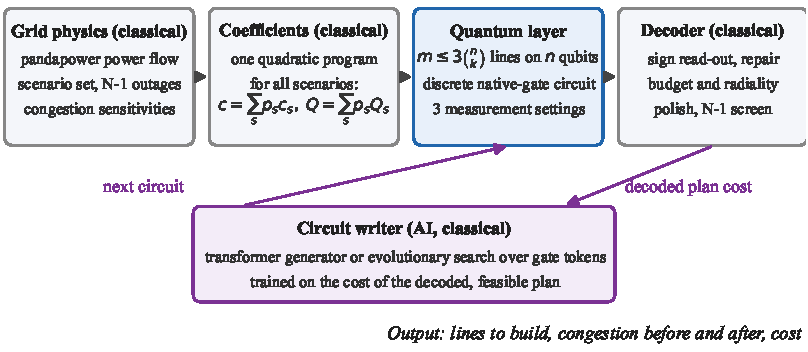
\includegraphics[width=\textwidth]{fig_workflow.pdf}
\caption{The hybrid loop. Everything that grows with the number of scenarios or
with the physics stays classical; the quantum layer sees one quadratic program
and returns $m$ correlation signs from three measurement settings.}
\label{fig:workflow}
\end{figure}

\subsection{From grid physics to one quadratic program}
Flows in Eq.~\eqref{eq:problem} are linear in injections for a fixed topology,
and the effect of adding candidate $e$ on the flow of line $l$ is a
line-outage-style sensitivity (the influence score of reference [4]). Expanding
the congestion term to second order in $x$ turns each scenario into a quadratic
binary program $c_s^{\top}x+x^{\top}Q_s x$, and because the build decision is
taken before the scenario is revealed, the expected objective is the single
program with $c=\sum_s p_s c_s$, $Q=\sum_s p_s Q_s$. That aggregation is exact
and classical, so \emph{scenario count costs nothing at the quantum layer}. We
have used this construction with thirteen weather scenarios clustered from
105,408 five-minute intervals of the RTS-GMLC dataset: the scenario set changed
the decision on 77.5\% of 40 instances and was strictly better under the
high-stress scenario on 77.5\% and worse on none, at identical qubits, depth
and shots. Coefficients came from a DC optimal power flow whose locational
price decomposition we verified numerically to $6.4\times10^{-4}$~\$/MWh. For
E.ON's medium- and low-voltage networks the same builder will read pandapower
models [10] (IEEE and CIGRE cases, SimBench feeders [11]) and use the linear
DistFlow branch model [12] on radial feeders, so voltage limits enter the
congestion term alongside thermal ratings.

\subsection{The encoding, and what it buys}
Each candidate line is assigned to one $k$-body Pauli string on the register.
Upgrade tiers on a corridor (for example three conductor sizes) are a monotone
chain of bits, a domain-wall encoding [9], chosen because an unconstrained bit
string is already a valid chain 97.5\% of the time against 13.8\% for plain
binary and 0\% for one-hot, and one bit flip moves the tier by exactly one
step. Table~\ref{tab:evidence} gives the measured compression: 7.5 decisions
per qubit at $m=45$, 15 at $m=105$, 600 at $m=9{,}009$. Over that range the
decision count grew 35.8-fold, the register 1.7-fold, and the measurement
cost not at all: three settings and $3\times1{,}024$ shots per circuit
evaluation at every size.

\subsection{Circuits written, not optimised}
The circuit is a sequence of tokens from a fixed vocabulary: single-qubit
rotations on a fixed angle grid, and either two-qubit entangling tokens or a
fixed brickwork of controlled-Z gates matching device connectivity. Two circuit
writers exist and both are gradient-free on the device:
\begin{itemize}
\item a decoder-only transformer in the style of the generative quantum
eigensolver [8], trained with a listwise preference loss on the cost of the
\emph{decoded, feasible} plan. Its one governing design quantity is the gate
budget: raising it from 19 to 59 gates lifted the share of 80 grid instances
solved to the certified optimum from 23.8\% to 48.8\% (paired Wilcoxon, better
on 45, worse on 4, $p=2.4\times10^{-7}$);
\item an elitist evolutionary search over the same token space, used at 60,
252 and 858 variables. Below 5,000 circuit executions it leads variational PCE
with parameter-shift gradients by 4 to 9 points of approximation ratio at
every size (Figure~\ref{fig:evidence}b); the variational method overtakes
only above $10^4$ to $10^5$ executions and needs 15 to 30 times the budget
for its final margin. The circuits contain no continuous
angle, need no compilation, and run unchanged on hardware.
\end{itemize}
The reward combines the exact decoded objective with the smoothed
$\tanh$ surrogate of [7]. We found that the surrogate is what makes decoded
signs survive finite shots: at 252 variables, circuits trained on the exact
objective alone kept an approximation ratio of 0.591 when read from 1,000
shots, against 0.698 with the smoothed term, because the latter drives
correlator magnitudes from 0.019 to 0.109. This is the design rule for the
hardware campaign in Section~5.

\subsection{Decoder: a feasible plan every time}
Sign read-out gives a bit string, not a plan. The decoder repairs each tier
chain, enforces the budget by removing the least valuable additions, checks
the topology rules, then polishes with a joint single- and pairwise-flip
search and a small integer program over the touched variables. Infeasible
output is structurally impossible: whatever the device returns, the planner
receives a buildable set of lines. Every decoded plan is then screened
classically against the full N-1 single-outage set with a security-constrained
power flow that is allowed to shed load, so the resilience effect of a plan is
a measured difference on identical outages. On IEEE-57 with 200~MW of added
load, the sited plan raised the share of outages served without shedding from
36.4\% to 96.1\% and cut expected unserved energy by 93.5\%.

\subsection{Qiskit compatibility layer, already in place}
Our PCE circuit-synthesis code base builds every circuit as a Qiskit
\texttt{QuantumCircuit}; the same three X/Y/Z measurement circuits run in the
exact statevector path and in Aer with and without noise models, and are
submitted unchanged to IBM hardware through the Qiskit Runtime path of the
library. Read-out is a Walsh-Hadamard transform of the
three count tables that returns all $m$ correlators at once, in
$O(n2^n)$ per basis and independent of $m$, and it agrees with Qiskit's Pauli
expectation values to $10^{-10}$. The grid package emits OpenQASM~3, which
Qiskit loads directly, and that is the path we used on Rigetti devices through
qBraid. E.ON can therefore execute and validate every result in Qiskit on day
one of the PoC, not at its end.

\begin{figure}[t]
\centering
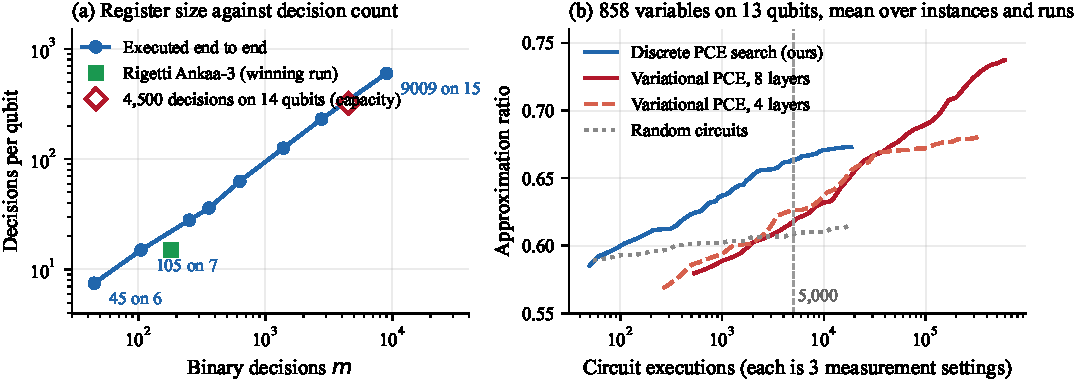
\includegraphics[width=\textwidth]{fig_evidence.pdf}
\caption{(a) Decisions per qubit across every configuration executed end to
end, the winning Ankaa-3 run, and the register a 4,500-decision planning
instance (500 corridors at nine upgrade tiers) would occupy. (b) Solution quality against quantum budget at 858
variables on 13 qubits, mean over instances and runs: the discrete PCE search
(no circuit parameters, no gradients) leads below 5,000 executions; the
variational method overtakes only after an order of magnitude more.}
\label{fig:evidence}
\end{figure}

% ---------------------------------------------------------------- 3
\section{Feasibility and Resource Requirements}

\textbf{Software.} Two public code bases exist and are the basis of the PoC.
\texttt{qGridX} (\url{\pypiurl}; \url{\qgridxurl}) is a pip-installable
package of 69 modules covering the power-flow layer, the encoding, the
transformer writer, the decoder, N-1 screening, statistics, and the hardware
path, with every published number reproduced by a one-line command and two
qBraid notebooks. \texttt{genpce} (6,758 lines, 26 unit tests) is the
Qiskit-native PCE circuit-synthesis library with the evolutionary writer, the
Walsh-Hadamard read-out, the variational baseline and the IBM Runtime path.
The PoC work is integration and a new coefficient builder, not new
infrastructure.

\textbf{Data.} Open only: pandapower IEEE and CIGRE medium- and low-voltage
cases, SimBench feeders, IEEE 33-, 69- and 123-bus radial systems, RTS-GMLC
time series for scenarios, and synthetic feeders generated to match their
graph statistics. E.ON's anonymised subgrids will be used when released, on
the same builder.

\textbf{Compute.} Exact simulation to 15 qubits runs on a laptop; the
9,009-decision instance took 30.4 hours on one 64-core cloud instance, which
is the largest exact run we will need. The 2,000-line rung fits 18 qubits at
$k=3$ and is exactly simulable. For the simulator study we deliberately use
$k=2$ on 24 to 30 qubits (828 to 1,305 line decisions): two-body correlators
are the largest and easiest to read on hardware, and a register above 24
qubits is where the question of Section~5 becomes meaningful; 30 qubits is the
top of exact statevector on one 64-core instance, and Aer's
matrix-product-state backend covers the rest. qBraid compute is already
provisioned.

\textbf{Hardware.} Rigetti through qBraid (we have run Ankaa-3 and
Cepheus-1-108Q) and IBM through Qiskit Runtime. Our measured costs set the
plan: one 1,024-shot job returns one measurement setting, so one circuit
evaluation is three jobs, and a 2,000-evaluation campaign is 6,000 short
jobs, submitted in batches. On Cepheus the $m=45$ and $m=105$ circuits routed
to 32 and 41 two-qubit gates at depth 58 and 81.

\textbf{Assumptions and constraints, stated.} (i) Flows are linearised (DC for
meshed medium voltage, linear DistFlow for radial low voltage); the decoder
re-evaluates every plan with a full pandapower power flow, so the linearisation
affects the search surface, not the reported objective. (ii) Scenarios are a
finite weighted set. (iii) Correlator magnitudes must clear the shot-noise
floor $1/\sqrt{N}\approx0.03$ to be read reliably, which sets a depth bar
that our device campaigns have located from both sides: two-qubit Bell
correlators on eight Cepheus edges came back at mean magnitudes 0.74 to 0.82
with 24 of 24 signs correct, while 59-gate generated circuits (32 two-qubit
gates after routing) fell below the floor. The hardware campaign therefore
opens with a depth sweep on the day's calibration, trains generated circuits
under the gate budget it locates, uses the smoothed term of Section~2.3, and
reads with measurement-error mitigation [14]. (iv) Exact simulation beyond
about 30 qubits is out of scope; above it the PoC uses hardware and
bounded-bond-dimension MPS only.

\textbf{Timeline.} Table~\ref{tab:plan} lays out sixteen weeks in five
overlapping work packages, each with a deliverable that exists as a file.

\begin{table}[t]
\centering
\caption{Work plan for the PoC sprint. Every deliverable is a file in the
public repository; WP1 is the challenge's stated foundation and is released
first so that E.ON and other teams can use it.}
\label{tab:plan}
\begin{tabularx}{\textwidth}{@{}lcX@{}}
\toprule
Work package & Weeks & Deliverable \\
\midrule
WP1 Hardness ladder & 1 to 4 & six instance sizes, $m=45$ to $2{,}000$, on open MV/LV networks; certified optima or best-known values; HiGHS and Gurobi time-to-optimality and root gap \\
WP2 Line-addition solver & 3 to 8 & pandapower coefficient builder, decoder rules for budget, tiers and radiality, simulation campaign to 15 qubits with all baselines and paired statistics \\
WP3 Hardware campaign & 7 to 12 & depth sweep, Bell controls, three-setting runs at $m=45$ and $m=105$ on Rigetti and IBM with mitigation; raw counts and analysis notebooks \\
WP4 Scale and simulator study & 9 to 14 & 24- to 30-qubit runs, MPS bond-dimension sweep, E.ON anonymised subgrids on the same builder, Qiskit validation package \\
WP5 Report and paper & 13 to 16 & reproducibility bundle with one command per figure, final report, joint paper draft with E.ON \\
\bottomrule
\end{tabularx}
\end{table}

% ---------------------------------------------------------------- 4
\section{Expected Impact}

A successful PoC demonstrates five things, each with a number attached.
\begin{enumerate}
\item \textbf{A hardness ladder for distribution expansion}, in the sense of
QOBLIB [5]: at least six instance sizes from $m=45$ to $m=2{,}000$ candidate
lines on open networks, each with a certified optimum or best-known value,
time-to-optimality for HiGHS and Gurobi, and root-gap, and at least one rung
at $m\le500$ where a commercial solver does not prove optimality within one
hour. This is the challenge's stated foundation and it is reusable by every
other team and by E.ON.
\item \textbf{A quantum workflow whose device workload does not grow with the
candidate set}: three measurement settings and a fixed shot budget from
$m=45$ to $m=2{,}000$, with the register between 6 and 30 qubits.
\item \textbf{Solution quality on the ladder.} Targets: the certified optimum
on at least 50\% of $m\le105$ instances at a matched 10,000-evaluation budget
(we reach 48.8\% on our transmission family today), and at least 0.95 of the
best-known value on $m\ge500$ instances within 20,000 evaluations.
\item \textbf{Hardware execution of at least one hard instance} at $m=45$ and
$m=105$ on a superconducting processor, with sign agreement against exact
simulation above 90\% after mitigation, and a decoded plan whose congestion
relief is within 10\% of the simulated one.
\item \textbf{A Qiskit-executable deliverable} that E.ON runs end to end in
under three hours per instance.
\end{enumerate}
For the use case, the change is from screening a handful of rule-based
reinforcement candidates to evaluating the joint choice over hundreds to
thousands of candidates across the full scenario set, with every plan
N-1-screened before it reaches a planner. E.ON's closing wish, a joint
scientific paper, is one we share: the ladder, the encoding and the device
measurements are each publishable on their own.

% ---------------------------------------------------------------- 5
\section{Validation Plan}

\textbf{Unit of analysis and statistics.} The unit is the instance, never the
run. Every comparison is paired on identical instances at a matched
evaluation budget and reported with a paired Wilcoxon signed-rank test for
objective values, McNemar's exact test for exact-match rates, and Wilson
intervals for proportions; at least 20 instances per rung. This is the
protocol behind every number quoted above.

\textbf{Baselines, all at matched budget.} Exact MIP (HiGHS, Gurobi academic
licence) with time-to-optimality; simulated annealing; tabu search; multi-start
greedy; random circuits through the same decoder (the ceiling the decoder can
extract from arbitrary input); variational PCE with parameter-shift gradients;
and one-qubit-per-variable QAOA on an extra $m\le30$ rung added for that
comparison, the only size at which it fits on hardware. On our current family the decoder-matched control ties our solver
($p=0.402$) and 20-restart greedy loses 62 instances to 2
($p=5.7\times10^{-12}$); we will publish the same table for the new ladder,
including the rungs where classical metaheuristics win.

\textbf{Metrics.} Congestion before and after (MW above rating, summed over
lines and scenarios, and the count of violated lines); investment cost;
approximation ratio to the certified or best-known value; share of instances
solved to the optimum; N-1 secure fraction and expected unserved energy of the
decoded plan; end-to-end wall clock.

\textbf{Hardware protocol.} Offline verification first: the emitted circuit is
executed two ways (package simulator and interpreted QASM) and must agree to
numerical precision, as it did before the Cepheus campaign (fidelity
$1.000000000000$, correlators to $3\times10^{-12}$). Then a Bell control on
every used edge, then the depth sweep, then the three settings per circuit
with read-out calibration in the same session. Reported quantities: sign agreement
and magnitude retention against exact simulation, both bit orderings, and the
decoded objective. Success is defined above; failure modes are reported with
the same tables.

\textbf{Secondary objective: simulator performance.} At $n\le20$ every circuit
is exactly simulable, so the MPS question is only meaningful on the 24- to
30-qubit rung. There we execute the trained circuits on Aer's
matrix-product-state backend at bond dimensions $\chi\in\{2,4,8,16,32,64\}$
and report the decoded congestion objective against the exact or hardware
value. Our trained PCE states are strongly entangled (half-chain entropy 2.1 of
3 bits at six qubits, all correlators between 0.13 and 0.37), so a
bounded-$\chi$ simulator is expected to degrade; the deliverable is the
measured $\chi$ at which it does, with confidence intervals.

\textbf{Reproducibility.} Seeds, CSV result files, one command per figure, and
qBraid notebooks, as in the two repositories today. Table~\ref{tab:success}
collects the criteria that define success.

\begin{table}[t]
\centering
\caption{Success criteria for the PoC. Each is measured by the protocol above
and reported whether or not it is met.}
\label{tab:success}
\begin{tabularx}{\textwidth}{@{}Xl@{}}
\toprule
Criterion & Target \\
\midrule
Hardness ladder released with certified values and solver times & 6 rungs; one rung at $m\le500$ unproven by Gurobi in 1 h \\
Device workload across the ladder & 3 settings, fixed shots, 6 to 30 qubits at every rung \\
Exact-match rate on $m\le105$ at 10,000 evaluations & $\ge50\%$ of instances (48.8\% today on the transmission family) \\
Ratio to best-known on $m\ge500$ at 20,000 evaluations & $\ge0.95$, paired against SA and tabu at the same budget \\
Hardware, $m=45$ and $m=105$ & sign agreement $\ge90\%$ after mitigation; decoded relief within 10\% of simulation \\
Simulator study, 24 to 30 qubits & bond dimension at which the MPS objective departs from exact, with CI \\
Qiskit execution by E.ON & end to end under 3 h per instance from the public package \\
\bottomrule
\end{tabularx}
\end{table}

% ---------------------------------------------------------------- 6
\section{Hybrid / Cross-Domain Integration}

The split in Figure~\ref{fig:workflow} is deliberate. Power-flow physics,
scenario aggregation and N-1 screening stay classical because they are linear
algebra that scales with grid size and scenario count, and none of it belongs
on a device. The AI layer, a transformer or an evolutionary search over gate
tokens, stays classical because that is where a learning signal can be
accumulated across thousands of proposals at no quantum cost, and because it
removes both the ansatz design problem and every quantum gradient. The device
does the one thing the classical layers cannot do cheaply: hold $m$ coupled
binary decisions as $m$ correlation signs of one entangled state and return
them from three measurements. The decoder closes the loop by guaranteeing
feasibility, so the quantum output is always a plan a planner can act on. The
same pipeline runs on a 64-core cloud instance with the device replaced by a
statevector or MPS simulator, which is how every rung of the ladder is
validated before device time is spent.

% ---------------------------------------------------------------- 7
\section{Team Capability}

\textbf{Track record on this exact method and this exact domain.} eQoSystem,
a team of AiQC (Ai and Quantum Community), won first place globally in the
Advanced Rigetti Computing Challenge at the Q-Volution hackathon hosted by
Girls in Quantum (March 2026), after being selected before the event for a
QPU access grant. The task was a 180-node weighted Max-Cut instance derived
from a real US power-grid topology; our PCE solution mapped the whole grid onto
12 qubits without partitioning, ran on the Rigetti Ankaa-3 QPU, and returned a
cut above the classical baseline. The Rigetti judges credited the team with
``a brilliant, deep understanding of the problem'' (\url{\blogurl};
solution at \url{\qvolrepo}). The team also represented Algeria and Africa at
MIT's iQuHACK 2026.

\textbf{Since then.} We built and published \texttt{qGridX} on PyPI, ran two
device campaigns on the Rigetti Cepheus-1-108Q through qBraid, wrote the PCE
circuit-synthesis library with its Qiskit Runtime path, and produced the
results in Table~\ref{tab:evidence}. Everything in Sections~2 to 5 is a
description of code we run, not of code we plan.

\textbf{Members.}
\begin{itemize}
\item \textbf{Achraf Boussahi} (lead). Co-director and Chief Scientific
Officer, AiQC; research intern, Constantine Quantum Technologies (CQTech);
ESI Sidi Bel Abbes. Quantum optimisation, PCE, hardware campaigns on Rigetti
Ankaa-3 and Cepheus-1-108Q, author of \texttt{qGridX} and of the DC-OPF and
N-1 layers.
\item \textbf{Abir Chekroun}. Co-director and Head of Quantum Projects, AiQC;
ESI Sidi Bel Abbes. Quantum algorithms and PCE pipelines; Q-Volution winning
team; quantum simulation packages.
\item \textbf{Zakaria Lourghi}. Co-director and Principal AI Engineer, AiQC;
ESI Sidi Bel Abbes. Transformer training, machine learning systems and
software engineering; Q-Volution winning team.
\item \textbf{Mouadh Abderrahmane Assal}. Co-director and Head of Advanced AI
Research, AiQC. Reinforcement learning and energy forecasting (renewable
energy forecasting datathon, quantum-assisted deep RL).
\item \textbf{Hiba Menacer}. \hibarole.
\end{itemize}
Quantum optimisation, power-system modelling, machine learning and software
delivery are each covered by at least one member who has shipped it, and the
lead has run every hardware platform the plan relies on.

% ---------------------------------------------------------------- refs
\vspace{4pt}
\hrule
\vspace{3pt}
{\color{eon}\bfseries References}
\begin{enumerate}[label={[\arabic*]},leftmargin=2em,itemsep=0pt]
\item G. Gust et al., ``Designing electricity
distribution networks: The impact of demand coincidence,'' \emph{European
Journal of Operational Research} 315(1), 271 to 288 (2024).
\item G. Duan, Y. Yu, ``Power distribution system optimization by an algorithm
for capacitated Steiner tree problems with complex-flows and arbitrary cost
functions,'' \emph{Int. J. Electrical Power and Energy Systems} 25(7), 515 to
523 (2003).
\item A. Khodabakhsh et al., ``A submodular approach for electricity
distribution network reconfiguration,'' arXiv:1711.03517 (2017).
\item J. J. Cuenca et al., ``Event-informed identification and allocation of
distribution network planning candidates with influence scores and binary
linear programming,'' \emph{IEEE Trans. Power Systems} 40(1), 492 to 504
(2024).
\item T. Koch et al., ``Quantum Optimization Benchmark Library: The
Intractable Decathlon,'' arXiv:2504.03832 (2025).
\item A. Kotil et al., ``Quantum approximate multi-objective optimization,''
\emph{Nature Computational Science} (2025).
\item M. Sciorilli, L. Borges, T. L. Patti, D. Garc\'ia-Mart\'in, G. Camilo,
A. Anandkumar, L. Aolita, ``Towards large-scale quantum optimization solvers
with few qubits,'' \emph{Nature Communications} 16, 476 (2025).
\item K. Nakaji et al., ``The generative quantum eigensolver (GQE) and its
application for ground state search,'' arXiv:2401.09253 (2024).
\item N. Chancellor, ``Domain wall encoding of discrete variables for quantum
annealing and QAOA,'' \emph{Quantum Science and Technology} 4, 045004 (2019).
\item L. Thurner et al., ``pandapower: An open-source Python tool for
convenient modeling, analysis, and optimization of electric power systems,''
\emph{IEEE Trans. Power Systems} 33(6), 6510 to 6521 (2018).
\item S. Meinecke et al., ``SimBench: A benchmark dataset of electric power
systems to compare innovative solutions based on power flow analysis,''
\emph{Energies} 13(12), 3290 (2020).
\item M. E. Baran, F. F. Wu, ``Network reconfiguration in distribution
systems for loss reduction and load balancing,'' \emph{IEEE Trans. Power
Delivery} 4(2), 1401 to 1407 (1989).
\item C. Barrows et al., ``The IEEE Reliability Test System: A proposed 2019
update,'' \emph{IEEE Trans. Power Systems} 35(1), 119 to 127 (2020).
\item P. D. Nation, H. Kang, N. Sundaresan, J. M. Gambetta, ``Scalable
mitigation of measurement errors on quantum computers,'' \emph{PRX Quantum}
2, 040326 (2021).
\end{enumerate}

\end{document}
